\subsection{基数0和1的性质}

命题6. 设 \((\mathfrak{a}_{\iota})_{\iota \in I}\) 为一族基数，并令 \(J\) （相应地，K）为 \(I\) 的一个子集，使得 \(\mathfrak{a}_{\iota} = 0\) （对于所有 \(\iota \notin J\) ）（相应地， \(\mathfrak{a}_{\iota} = 1\) 对于所有 \(\iota \notin K\) ）。则

\[
\sum_ {i \in I} a _ {i} = \sum_ {i \in J} a _ {i} \quad \left(\text { 分别 } \underset {i \in I} {\mathbf {P}} a _ {i} = \underset {i \in K} {\mathbf {P}} a _ {i}\right).
\]

该命题对于和来说是显然的，因为和 \(S_{I}\) （集合族 \((a_{i})_{i\in I}\) 的和）与 \(S_{J}\) （族 \((a_{i})_{i\in I}\) 的和）与空集的并集等势，因此与 \(S_{J}\) 等势。关于乘积的断言由以下事实得出：投影 \(pr_{K}\) （乘积集合 \(\prod_{i\in I} a_{i}\) 到部分乘积 \(\prod_{i\in K} a_{i}\) 上的投影）是一个双射（第二章，§5，第5号，注记1）。

推论1. 对于每一个基数a，我们有 \(a + 0 = a\) . \(1 = a\) .

推论2。设 \(\mathfrak{a}\) 与 \(\mathfrak{b}\) 是基数，且令 \(\mathbf{I}\) 是一个与 \(\mathfrak{b}\) 等势的集合。对于每一个 \(\iota \in \mathbf{I}\) ，令 \(\mathfrak{a}_t = \mathfrak{a}, \mathfrak{c}_t = 1\) 。则

\[
\mathfrak {a}\mathfrak {b} = \sum_ {i \in I} \mathfrak {a} _ {i}, \quad \mathfrak {b} = \sum_ {i \in I} \mathfrak {c} _ {i}.
\]

第二个公式是由任何集合都是其单元素子集的并集这一事实得出的。第一个公式由第二个公式两端乘以 \(\mathfrak{a}\) 并利用推论1得出。

命题7。设 \((\mathfrak{a}_{i})_{i\in I}\) 为一个基数族。则 \(\underset{i\in I}{\mathsf{P}}\mathfrak{a}_{i}\neq 0\) 当且仅当 \(\mathfrak{a}_i\neq 0\) （对于所有 \(i\in I\) ）.

这仅仅是乘积集应为非空这一条件的翻译（第二章，§5，第4号，命题5，推论2）。

命题8。若 \(\mathfrak{a}\) 与 \(\mathfrak{b}\) 是基数，使得 \(\mathfrak{a} + 1 = \mathfrak{b} + 1\) ，那么 \(\mathfrak{a} = \mathfrak{b}\) .

令 \(X = a + 1 = b + 1\) 。则存在 X 的子集 A、B，其基数分别为 \(a, b\) ，使得补集 X ＼ A、X ＼ B 各只含一个元素。设 u、v 分别为这些元素。交集 \(C = A \cap B\) 在 X 中的补集为集合 \(\{u, v\}\) 。若 u = v，则 A = B = C，从而 \(a = b\) 。如果 \(u \neq v\) ，则 A = C ∪ \(\{v\}\) ，B = C ∪ \(\{u\}\) ，从而 \(a = 1 + \text{Card (C)} = b\) .

\pandocbounded{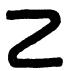
\includegraphics[keepaspectratio]{images/part002_ad0e6982551a0008e23df60b46a8b3d8f866f5ecbe9521df85283d9b8fea8d5c.jpg}}

读者应注意不要假定 \(a + m = b + m\) 对所有基数 m 都蕴含 a = b（参见 §6）；* 然而我们稍后将看到，若 m 是有限的，则这一蕴含关系成立（§5，第 2 号，命题 3，推论 4 以及 §6，第 3 号，定理 3，推论 4）。*

